\documentclass{standalone}
\usepackage{pgfplots}
\pgfplotsset{compat=newest}
\begin{document}
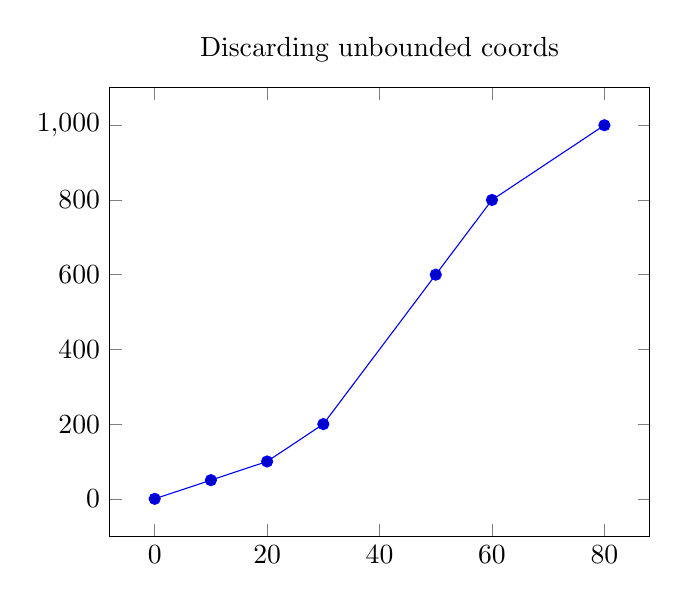
\begin{tikzpicture}
\begin{axis}[
	title=Discarding unbounded coords,
	unbounded coords=discard]
	\addplot coordinates {
		(0,0) (10,50) (20,100) (30,200) 
		(40,inf) (50,600) (60,800) (80,1000)
	};
\end{axis}
\end{tikzpicture}
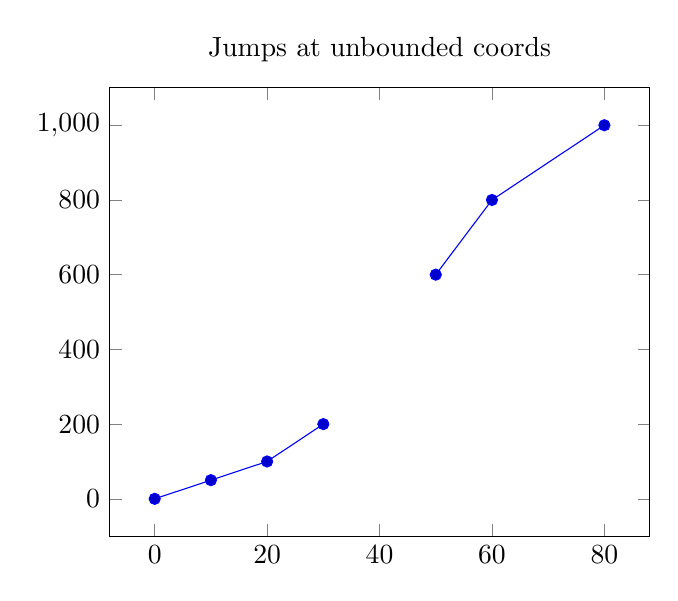
\begin{tikzpicture}
\begin{axis}[
	title=Jumps at unbounded coords,
	unbounded coords=jump]
	\addplot coordinates {
		(0,0) (10,50) (20,100) (30,200) 
		(40,inf) (50,600) (60,800) (80,1000)
	};
\end{axis}
\end{tikzpicture}
\end{document}
